\documentclass[10pt,a4paper]{article}
\usepackage[a4paper,top=19mm,bottom=18mm,left=20mm,right=20mm,footskip=9mm]{geometry}
\usepackage{fontspec,xcolor,tikz,tcolorbox,tabularx,booktabs,enumitem,fancyhdr,microtype}
\usepackage{graphicx}
\special{dvipdfmx:config z 0}   % ohne Kompression, maximale Druckkompatibilitaet
\usetikzlibrary{arrows.meta,shadows.blur,fit}
\tcbuselibrary{skins}
\usepackage[ngerman,provide=*]{babel}
\usepackage{hyperref}\hypersetup{hidelinks,pdftitle={Pending Orders – Kurz-Guide},pdfsubject={Buy Limit, Sell Limit, Buy Stop, Sell Stop}}

\setmainfont{IBMPlexSans-Regular.otf}[Path=/root/.fonts/,
  BoldFont={IBMPlexSans-SemiBold.otf}, ItalicFont={IBMPlexSans-Italic.otf},
  BoldItalicFont={IBMPlexSans-SemiBoldItalic.otf}]
\newfontfamily\light{IBMPlexSans-Light.otf}[Path=/root/.fonts/,
  BoldFont={IBMPlexSans-Regular.otf}, ItalicFont={IBMPlexSans-LightItalic.otf}]
\newfontfamily\mono{IBMPlexMono-Regular.otf}[Path=/root/.fonts/,
  BoldFont={IBMPlexMono-SemiBold.otf}]
\newcommand{\num}[1]{{\mono #1}}

% ---- Farben -------------------------------------------------------------
\definecolor{ink}{HTML}{14161A}    \definecolor{body}{HTML}{3C4249}
\definecolor{muted}{HTML}{6D757E}  \definecolor{soft}{HTML}{9AA1AA}
\definecolor{rule}{HTML}{E2E5E9}   \definecolor{greya}{HTML}{A8AEB6}
\definecolor{buy}{HTML}{0E7A4E}    \definecolor{sell}{HTML}{B23A2E}
\definecolor{buytint}{HTML}{E9F4EE} \definecolor{selltint}{HTML}{FAEDEB}
\definecolor{paper}{HTML}{F7F8F9}
\definecolor{pfbg}{HTML}{001328}\definecolor{pfgruen}{HTML}{0E7A4E}
\definecolor{pfgrau}{HTML}{97A5B4}\definecolor{pfrot}{HTML}{B23A2E}
\definecolor{pfgrey}{HTML}{6A6A6A}
\definecolor{wbg}{HTML}{0E2939} \definecolor{whead}{HTML}{0B2130} \definecolor{wfield}{HTML}{102B3C}
\definecolor{wborder}{HTML}{1D4256} \definecolor{waccent}{HTML}{1B6CA8} \definecolor{wgreen}{HTML}{3CB44A}
\definecolor{wtext}{HTML}{E7EEF2} \definecolor{wmuted}{HTML}{8FA6B3} \definecolor{wmark}{HTML}{3F88BD}
\definecolor{wdim}{HTML}{5F7A89} \definecolor{wtog}{HTML}{33505F} \definecolor{wknob}{HTML}{C3D2DA}
\definecolor{wred}{HTML}{E0524D} \definecolor{wchart}{HTML}{0B2030} \definecolor{wpill}{HTML}{5B6B76}
\definecolor{wtabtext}{HTML}{CDDBE3} \definecolor{wbadge}{HTML}{0B3A17}

% ---- Typografische Skala (1,25) -----------------------------------------
\newcommand{\display}{\light\fontsize{30}{34}\selectfont}
\newcommand{\hone}{\fontsize{19}{23}\selectfont\bfseries}
\newcommand{\htwo}{\fontsize{8}{11}\selectfont\bfseries}
\newcommand{\hthree}{\fontsize{12}{15}\selectfont\bfseries}
\newcommand{\leadf}{\light\fontsize{11.5}{17}\selectfont}
\renewcommand{\small}{\fontsize{8.6}{12.4}\selectfont}
\newcommand{\lbl}{\fontsize{7.6}{10}\selectfont}
\newcommand{\micro}{\fontsize{7}{9}\selectfont}
\newcommand{\wfont}{\fontsize{6.8}{8}\selectfont}
\newcommand{\wsmall}{\fontsize{5.8}{7}\selectfont}
\newcommand{\fine}{\fontsize{7.4}{9.2}\selectfont}
\newcommand{\foot}{\fontsize{6.2}{7.6}\selectfont}
\newcommand{\ls}{\addfontfeatures{LetterSpace=14}}
\newcommand{\lsx}{\addfontfeatures{LetterSpace=8}}
\normalsize\fontsize{9.4}{14}\selectfont
\color{body}\setlength{\parindent}{0pt}\setlength{\parskip}{0pt}
\setlength{\emergencystretch}{2em}
\hyphenpenalty=400\relax

% ---- Bausteine ----------------------------------------------------------
\newcommand{\kicker}[2]{{\htwo\ls\color{muted}\MakeUppercase{#2}\par}%
  \vspace{2mm}{\color{rule}\rule{\linewidth}{0.4pt}}\par\vspace{5.5mm}}
\newcommand{\Hone}[1]{{\hone\color{ink}#1\par}\vspace{3.5mm}}
\newcommand{\Htwo}[1]{{\htwo\ls\color{muted}\MakeUppercase{#1}\par}\vspace{4mm}}
\newcommand{\lead}[1]{{\leadf\color{body}\raggedright #1\par}}
\newcommand{\hr}{\par\vspace{7mm}{\color{rule}\rule{\linewidth}{0.4pt}}\par\vspace{6mm}}
\newcommand{\hd}[1]{{\micro\bfseries\ls\color{soft}\MakeUppercase{#1}}}
\tikzset{cnum/.style={circle,fill=ink,text=white,inner sep=0,minimum size=3.2mm,
  font=\bfseries\fontsize{5.6}{6}\selectfont}}
\newcommand{\cn}[1]{\tikz[baseline=-0.65ex]\node[cnum]{#1};}
\tikzset{pfnum/.style={circle,fill=ink,text=white,inner sep=0,minimum size=13,
  font=\bfseries\fontsize{7}{8}\selectfont}}
\newcommand{\pflab}{\fontsize{7}{8.5}\selectfont}
\newcommand{\pfn}[1]{\tikz[baseline=-0.7ex]\node[circle,fill=ink,text=white,inner sep=0,
  minimum size=4.4mm,font=\bfseries\fontsize{7}{8}\selectfont]{#1};}
\usetikzlibrary{calc}
\input{charts.tikz}
% weicher Schatten fuer eingebundene Grafiken
\tikzset{softshadow/.style={blur shadow={shadow blur steps=16,shadow xshift=0pt,
  shadow yshift=-0.9pt,shadow opacity=30,shadow blur radius=1.5mm}}}
\newcommand{\shadowfig}[2][80mm]{%
  \tikz[baseline=(current bounding box.north)]\node[inner sep=0,softshadow]
    {\includegraphics[width=#1]{#2}};}

\newtcolorbox{merk}{enhanced,colback=paper,colframe=paper,boxrule=0pt,arc=0pt,
  borderline west={2pt}{0pt}{ink},left=5mm,right=5mm,top=3.5mm,bottom=3.5mm,boxsep=0pt,
  before skip=6mm,after skip=0pt,fontupper=\small\color{body}}
\newtcolorbox{prule}[1]{enhanced,colback=white,colframe=rule,boxrule=0.4pt,arc=1mm,
  borderline west={2pt}{0pt}{#1},left=4mm,right=4mm,top=2.6mm,bottom=2.6mm,boxsep=0pt,
  before skip=2.2mm,after skip=0pt,fontupper=\small\color{body}}
\newtcolorbox{soft}{enhanced,colback=paper,colframe=paper,boxrule=0pt,arc=1.5mm,
  left=5mm,right=5mm,top=4mm,bottom=4mm,boxsep=0pt,before skip=0pt,after skip=0pt,
  before upper={\raggedright\hyphenpenalty=10000\relax\exhyphenpenalty=10000\relax}}

\pagestyle{fancy}\fancyhf{}\renewcommand{\headrulewidth}{0pt}

\fancyfoot[L]{\micro\color{soft}\ls PENDING ORDERS · KURZ-GUIDE}
\begin{document}
\thispagestyle{empty}
{\htwo\ls\color{muted}TRADING-GRUNDLAGEN}\par\vspace{11mm}
{\display\color{ink}Pending Orders}\par\vspace{7mm}
{\color{ink}\rule{28mm}{2pt}}\par\vspace{6mm}
\begin{minipage}{124mm}\lead{Die vier Ordertypen auf einen Blick – damit du Einstieg,
Auslösepreis und Richtung richtig kombinierst.}\end{minipage}
\par\vspace{6mm}
\tikz\node[draw=rule,line width=0.4pt,rounded corners=1.6mm,inner xsep=3mm,inner ysep=1.5mm,
  text=muted,font=\micro\bfseries\ls]{4 ORDERTYPEN. 1 KLARE ENTSCHEIDUNGSLOGIK.};
\par\vspace{0pt plus 1fill}
\noindent\begin{tikzpicture}[x=1mm,y=1mm]
\useasboundingbox (0,0) rectangle (170.0,130.8);
\node[inner sep=0,text=muted,font=\lbl\bfseries\ls] at (85.0,126.8) {AT PRICE ÜBER DEM AKTUELLEN KURS};
\node[inner sep=0,text=muted,font=\lbl\bfseries\ls] at (85.0,4) {AT PRICE UNTER DEM AKTUELLEN KURS};
\draw[body,line width=0.7pt] (0,65.37931034482759) -- (170.0,65.37931034482759);
\node[inner sep=0,fill=white,inner xsep=3.2mm,text=ink,font=\lbl\bfseries\ls] at (85.0,65.37931034482759) {KURS JETZT};
\begin{scope}[shift={(19.50,95.38)},scale=0.26437]
\chartbsmini
\end{scope}
\node[inner sep=0,text=buy,font=\hthree] at (42.50,85.88) {BUY STOP};
\node[inner sep=0,text=muted,font=\small] at (42.50,79.88) {Ausbruch nach oben};
\begin{scope}[shift={(104.50,95.38)},scale=0.26437]
\chartslmini
\end{scope}
\node[inner sep=0,text=sell,font=\hthree] at (127.50,85.88) {SELL LIMIT};
\node[inner sep=0,text=muted,font=\small] at (127.50,79.88) {teurer verkaufen};
\begin{scope}[shift={(19.50,10.00)},scale=0.26437]
\chartblmini
\end{scope}
\node[inner sep=0,text=buy,font=\hthree] at (42.50,50.88) {BUY LIMIT};
\node[inner sep=0,text=muted,font=\small] at (42.50,44.88) {günstiger kaufen};
\begin{scope}[shift={(104.50,10.00)},scale=0.26437]
\chartssmini
\end{scope}
\node[inner sep=0,text=sell,font=\hthree] at (127.50,50.88) {SELL STOP};
\node[inner sep=0,text=muted,font=\small] at (127.50,44.88) {Ausbruch nach unten};
\end{tikzpicture}
\par\vspace{0pt plus 1.35fill}
{\color{rule}\rule{\linewidth}{0.4pt}}\par\vspace{2.5mm}
{\micro\ls\color{soft}PENDING ORDERS\hfill KURZ-GUIDE}
\clearpage
\kicker{}{Fundament}
\Hone{Was eine Pending Order ist}
\begin{minipage}{128mm}\lead{Du kaufst oder verkaufst nicht sofort. Du legst vorher einen Kurs fest –
und die Plattform wartet für dich, bis er erreicht ist.}\end{minipage}
\par\vspace{8mm}
\noindent\begin{minipage}[t]{82mm}\vspace{0pt}\begin{soft}
{\htwo\ls\color{muted}NEW MARKET ORDER}\par\vspace{2mm}
{\hthree\color{ink}Sofort.}\par\vspace{1.5mm}
{\color{body}Du klickst – und der Kauf oder Verkauf passiert im selben Moment,
zum Kurs, der gerade gilt.}\end{soft}\end{minipage}\hfill
\begin{minipage}[t]{82mm}\vspace{0pt}\begin{soft}
{\htwo\ls\color{muted}NEW PENDING ORDER}\par\vspace{2mm}
{\hthree\color{ink}Später.}\par\vspace{1.5mm}
{\color{body}Du trägst bei At price deinen Aktivierungspunkt ein. Erreicht der Markt ihn,
wird die Order ausgelöst.}\end{soft}\end{minipage}
\hr
\Htwo{Der aktuelle Kurs ist dein Nullpunkt}
{\color{body}Jeder Wert, den du bei At price einträgst, liegt entweder über oder unter dem Kurs
von jetzt. Genau daran erkennst du, welchen Ordertyp du brauchst.}\par\vspace{6mm}
\noindent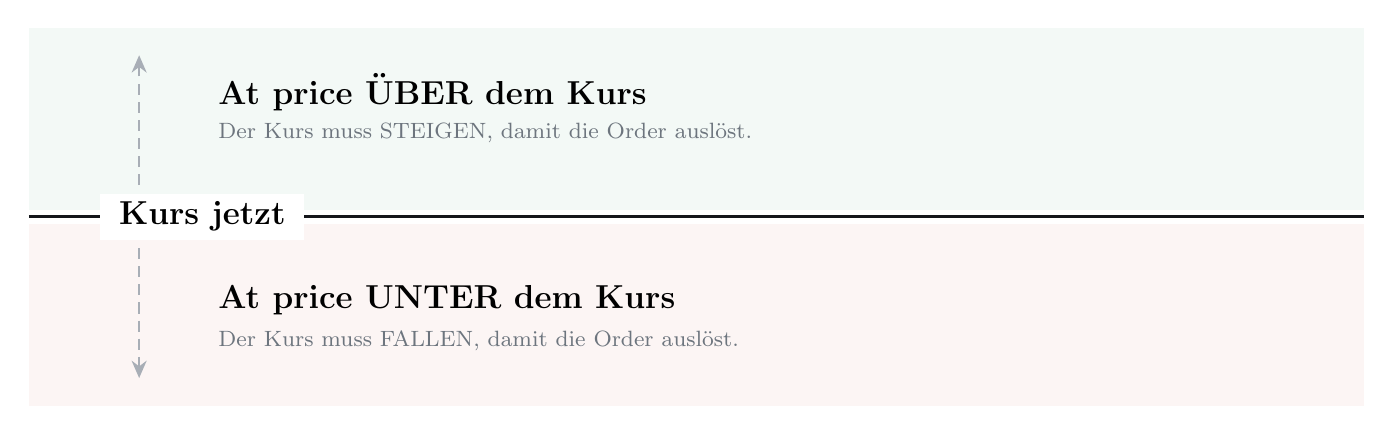
\begin{tikzpicture}[x=1mm,y=1mm,font=\lbl]
\fill[buytint,opacity=0.55] (0,0.9) rectangle (169.5,24.0);
\fill[selltint,opacity=0.55] (0,-24.0) rectangle (169.5,-0.9);
\draw[ink,line width=0.9pt] (0,0) -- (169.5,0);
\node[anchor=west,inner sep=0,font=\hthree] at (9,0) {\colorbox{white}{\;Kurs jetzt\;}};
\draw[greya,line width=0.8pt,dash pattern=on 1.4mm off 0.9mm,-{Stealth[length=2.2mm,width=1.9mm]}] (14,4) -- (14,20.5);
\node[anchor=west,inner sep=0,font=\hthree] at (24,15.8) {At price ÜBER dem Kurs};
\node[anchor=west,inner sep=0,text=muted] at (24,10.600000000000001) {Der Kurs muss STEIGEN, damit die Order auslöst.}; 
\draw[greya,line width=0.8pt,dash pattern=on 1.4mm off 0.9mm,-{Stealth[length=2.2mm,width=1.9mm]}] (14,-4) -- (14,-20.5);
\node[anchor=west,inner sep=0,font=\hthree] at (24,-10.600000000000001) {At price UNTER dem Kurs};
\node[anchor=west,inner sep=0,text=muted] at (24,-15.8) {Der Kurs muss FALLEN, damit die Order auslöst.}; 
\end{tikzpicture}
\par\vspace{4mm}
{\color{muted}\small Kaufen und unter dem Kurs: \textcolor{buy}{\bfseries Buy Limit}.
Kaufen und über dem Kurs: \textcolor{buy}{\bfseries Buy Stop}.
Verkaufen und über dem Kurs: \textcolor{sell}{\bfseries Sell Limit}.
Verkaufen und unter dem Kurs: \textcolor{sell}{\bfseries Sell Stop}.}
\hr
\Htwo{Warum im Voraus planen}
\noindent\begin{minipage}[t]{53mm}\vspace{0pt}\raggedright
{\bfseries Du musst nicht am Bildschirm sitzen.}\par\vspace{1mm}
{\color{muted}\small Die Plattform wartet für dich – auch nachts oder während du arbeitest.}
\end{minipage}\hfill
\begin{minipage}[t]{53mm}\vspace{0pt}\raggedright
{\bfseries Du entscheidest in Ruhe.}\par\vspace{1mm}
{\color{muted}\small Den Kurs legst du vorher fest – nicht in dem Moment, in dem sich der Markt bewegt.}
\end{minipage}\hfill
\begin{minipage}[t]{53mm}\vspace{0pt}\raggedright
{\bfseries Sie löst nur bei deinem Wert aus.}\par\vspace{1mm}
{\color{muted}\small Nicht früher. Du läufst dem Kurs nicht hinterher.}
\end{minipage}
\clearpage
\kicker{}{Die Limit-Typen}
\Hone{Limit wartet auf den besseren Kurs}
\begin{minipage}{125mm}\lead{Bei Limit liegt dein At-price-Wert dort, wo du einen günstigeren
Preis bekommst als jetzt. Erreicht der Markt deinen Aktivierungspunkt, wird die Order ausgelöst.}\end{minipage}
\par\vspace{10mm}

{\hthree\color{buy}BUY LIMIT}\hfill
{\fine\color{muted}günstiger kaufen · At price liegt unter dem Kurs}\par\vspace{1.4mm}
{\color{rule}\rule{\linewidth}{0.4pt}}\par\vspace{5mm}
\noindent\begin{minipage}[t]{94mm}\vspace{0pt}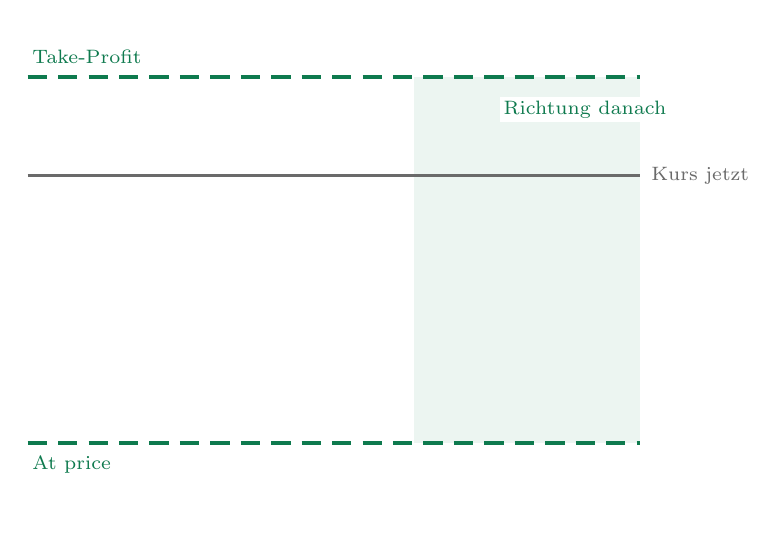
\begin{tikzpicture}[x=0.44660mm,y=0.44660mm]
\useasboundingbox (0,-10) rectangle (206,126);
\fill[pfgruen,opacity=0.08] (110,8) rectangle (174,112);
\draw[pfgruen,line width=1.5,dash pattern=on 7 off 4] (0,112) -- (174,112);
\node[anchor=south west,inner sep=1.5,fill=white,text=pfgruen] at (0,114.5) {\pflab Take-Profit};
\draw[pfgruen,line width=1.5,dash pattern=on 7 off 4] (0,8) -- (174,8);
\node[anchor=north west,inner sep=1.5,fill=white,text=pfgruen] at (0,5.5) {\pflab At price};
\draw[pfgrey,line width=0.9] (0,84) -- (174,84);
\node[anchor=west,inner sep=1.5,fill=white,text=pfgrey] at (176,84) {\pflab Kurs jetzt};
\chartbl
\node[anchor=south,inner sep=1.5,fill=white,text=pfgruen] at (158.5,99) {\pflab Richtung danach};
\end{tikzpicture}\end{minipage}\hfill
\begin{minipage}[t]{72mm}\vspace{1mm}\raggedright
{\bfseries\color{ink}Kurs jetzt}\par{\color{muted}\small Die graue Linie ist der Kurs in dem Moment, in dem du die Order aufgibst. Die rote Kugel zeigt genau diesen Punkt.}\par\vspace{3.8mm}
{\bfseries\color{pfgruen}At price}\par{\color{muted}\small Dein Aktivierungspunkt, hier \textbf{unter} dem Kurs. Erreicht der Markt ihn, wird die Order ausgelöst. Bis dahin passiert nichts.}\par\vspace{3.8mm}
{\bfseries\color{pfgruen}Richtung danach}\par{\color{muted}\small Das Dreieck zeigt, wohin es dann gehen soll: der Kurs soll \textbf{steigen} – bis zu deinem Take-Profit.}\par\vspace{3.8mm}
{\bfseries\color{ink}Wann sinnvoll}\par{\color{muted}\small Wenn du glaubst, der Kurs fällt kurz zurück, bevor er steigt. Du kaufst dann günstiger als jetzt.}
\end{minipage}\par
\hr

{\hthree\color{sell}SELL LIMIT}\hfill
{\fine\color{muted}teurer verkaufen · At price liegt über dem Kurs}\par\vspace{1.4mm}
{\color{rule}\rule{\linewidth}{0.4pt}}\par\vspace{5mm}
\noindent\begin{minipage}[t]{94mm}\vspace{0pt}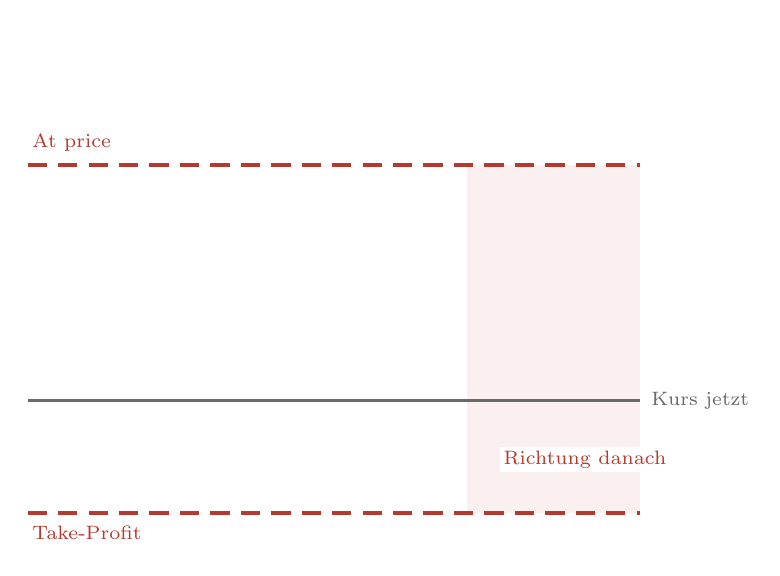
\begin{tikzpicture}[x=0.44660mm,y=0.44660mm]
\useasboundingbox (0,-26) rectangle (206,122);
\fill[pfrot,opacity=0.08] (125,-16) rectangle (174,83);
\draw[pfrot,line width=1.5,dash pattern=on 7 off 4] (0,-16) -- (174,-16);
\node[anchor=north west,inner sep=1.5,fill=white,text=pfrot] at (0,-18.5) {\pflab Take-Profit};
\draw[pfrot,line width=1.5,dash pattern=on 7 off 4] (0,83) -- (174,83);
\node[anchor=south west,inner sep=1.5,fill=white,text=pfrot] at (0,85.5) {\pflab At price};
\draw[pfgrey,line width=0.9] (0,16) -- (174,16);
\node[anchor=west,inner sep=1.5,fill=white,text=pfgrey] at (176,16) {\pflab Kurs jetzt};
\chartsl
\node[anchor=north,inner sep=1.5,fill=white,text=pfrot] at (158.5,3) {\pflab Richtung danach};
\end{tikzpicture}\end{minipage}\hfill
\begin{minipage}[t]{72mm}\vspace{1mm}\raggedright
{\bfseries\color{ink}Kurs jetzt}\par{\color{muted}\small Die graue Linie ist der Kurs in dem Moment, in dem du die Order aufgibst. Die rote Kugel zeigt genau diesen Punkt.}\par\vspace{3.8mm}
{\bfseries\color{pfrot}At price}\par{\color{muted}\small Dein Aktivierungspunkt, hier \textbf{über} dem Kurs. Erreicht der Markt ihn, wird die Order ausgelöst. Bis dahin passiert nichts.}\par\vspace{3.8mm}
{\bfseries\color{pfrot}Richtung danach}\par{\color{muted}\small Das Dreieck zeigt, wohin es dann gehen soll: der Kurs soll \textbf{fallen} – bis zu deinem Take-Profit.}\par\vspace{3.8mm}
{\bfseries\color{ink}Wann sinnvoll}\par{\color{muted}\small Wenn du glaubst, der Kurs steigt noch ein Stück, bevor er fällt. Du verkaufst dann teurer als jetzt.}
\end{minipage}\par
\clearpage
\kicker{}{Die Stop-Typen}
\Hone{Stop wartet auf die Bewegung}
\begin{minipage}{125mm}\lead{Bei Stop liegt dein At-price-Wert auf der ungünstigeren Seite.
Die Order löst erst aus, wenn der Kurs durch den Wert bricht – du steigst also erst ein, wenn
die Bewegung schon da ist.}\end{minipage}
\par\vspace{10mm}

{\hthree\color{buy}BUY STOP}\hfill
{\fine\color{muted}Ausbruch nach oben kaufen · At price liegt über dem Kurs}\par\vspace{1.4mm}
{\color{rule}\rule{\linewidth}{0.4pt}}\par\vspace{5mm}
\noindent\begin{minipage}[t]{94mm}\vspace{0pt}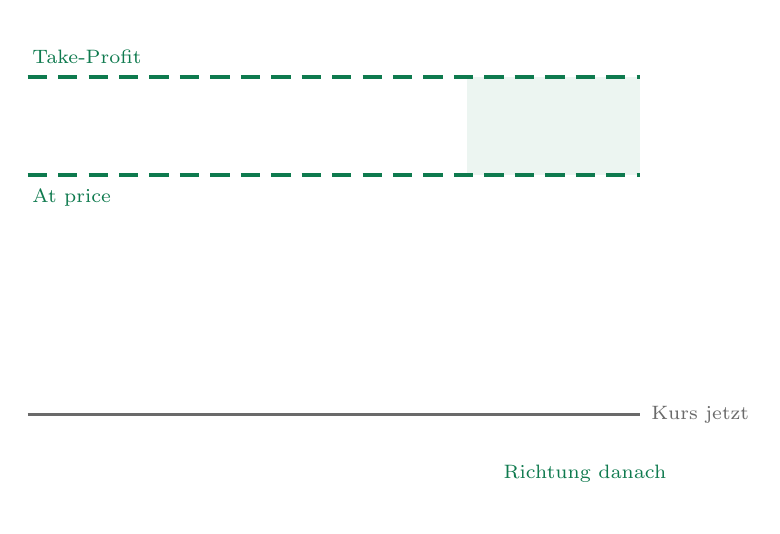
\begin{tikzpicture}[x=0.44660mm,y=0.44660mm]
\useasboundingbox (0,-10) rectangle (206,126);
\fill[pfgruen,opacity=0.08] (125,84) rectangle (174,112);
\draw[pfgruen,line width=1.5,dash pattern=on 7 off 4] (0,112) -- (174,112);
\node[anchor=south west,inner sep=1.5,fill=white,text=pfgruen] at (0,114.5) {\pflab Take-Profit};
\draw[pfgruen,line width=1.5,dash pattern=on 7 off 4] (0,84) -- (174,84);
\node[anchor=north west,inner sep=1.5,fill=white,text=pfgruen] at (0,81.5) {\pflab At price};
\draw[pfgrey,line width=0.9] (0,16) -- (174,16);
\node[anchor=west,inner sep=1.5,fill=white,text=pfgrey] at (176,16) {\pflab Kurs jetzt};
\chartbs
\node[anchor=north,inner sep=1.5,fill=white,text=pfgruen] at (158.5,3) {\pflab Richtung danach};
\end{tikzpicture}\end{minipage}\hfill
\begin{minipage}[t]{72mm}\vspace{1mm}\raggedright
{\bfseries\color{ink}Kurs jetzt}\par{\color{muted}\small Die graue Linie ist der Kurs in dem Moment, in dem du die Order aufgibst. Die rote Kugel zeigt genau diesen Punkt.}\par\vspace{3.8mm}
{\bfseries\color{pfgruen}At price}\par{\color{muted}\small Dein Aktivierungspunkt, hier \textbf{über} dem Kurs. Erreicht der Markt ihn, wird die Order ausgelöst. Bis dahin passiert nichts.}\par\vspace{3.8mm}
{\bfseries\color{pfgruen}Richtung danach}\par{\color{muted}\small Das Dreieck zeigt, wohin es dann gehen soll: der Kurs soll \textbf{steigen} – bis zu deinem Take-Profit.}\par\vspace{3.8mm}
{\bfseries\color{ink}Wann sinnvoll}\par{\color{muted}\small Wenn du erst kaufen willst, sobald der Kurs eine Hürde nach oben genommen hat – nicht vorher.}
\end{minipage}\par
\hr

{\hthree\color{sell}SELL STOP}\hfill
{\fine\color{muted}Ausbruch nach unten verkaufen · At price liegt unter dem Kurs}\par\vspace{1.4mm}
{\color{rule}\rule{\linewidth}{0.4pt}}\par\vspace{5mm}
\noindent\begin{minipage}[t]{94mm}\vspace{0pt}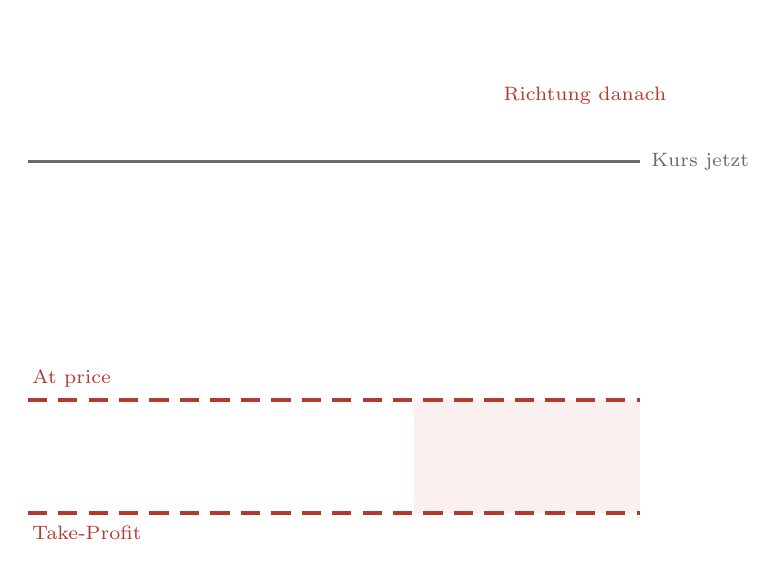
\begin{tikzpicture}[x=0.44660mm,y=0.44660mm]
\useasboundingbox (0,-26) rectangle (206,122);
\fill[pfrot,opacity=0.08] (110,-16) rectangle (174,16);
\draw[pfrot,line width=1.5,dash pattern=on 7 off 4] (0,-16) -- (174,-16);
\node[anchor=north west,inner sep=1.5,fill=white,text=pfrot] at (0,-18.5) {\pflab Take-Profit};
\draw[pfrot,line width=1.5,dash pattern=on 7 off 4] (0,16) -- (174,16);
\node[anchor=south west,inner sep=1.5,fill=white,text=pfrot] at (0,18.5) {\pflab At price};
\draw[pfgrey,line width=0.9] (0,84) -- (174,84);
\node[anchor=west,inner sep=1.5,fill=white,text=pfgrey] at (176,84) {\pflab Kurs jetzt};
\chartss
\node[anchor=south,inner sep=1.5,fill=white,text=pfrot] at (158.5,99) {\pflab Richtung danach};
\end{tikzpicture}\end{minipage}\hfill
\begin{minipage}[t]{72mm}\vspace{1mm}\raggedright
{\bfseries\color{ink}Kurs jetzt}\par{\color{muted}\small Die graue Linie ist der Kurs in dem Moment, in dem du die Order aufgibst. Die rote Kugel zeigt genau diesen Punkt.}\par\vspace{3.8mm}
{\bfseries\color{pfrot}At price}\par{\color{muted}\small Dein Aktivierungspunkt, hier \textbf{unter} dem Kurs. Erreicht der Markt ihn, wird die Order ausgelöst. Bis dahin passiert nichts.}\par\vspace{3.8mm}
{\bfseries\color{pfrot}Richtung danach}\par{\color{muted}\small Das Dreieck zeigt, wohin es dann gehen soll: der Kurs soll \textbf{fallen} – bis zu deinem Take-Profit.}\par\vspace{3.8mm}
{\bfseries\color{ink}Wann sinnvoll}\par{\color{muted}\small Wenn du erst verkaufen willst, sobald der Kurs nach unten durchbricht – nicht vorher.}
\end{minipage}\par
\clearpage
\kicker{}{Spickzettel}
\Hone{Alle vier nebeneinander}
\begin{minipage}{128mm}\lead{Vier Bilder, ein Muster: Die rote Kugel ist der Kurs, wenn du die Order
aufgibst. Die grüne Kugel ist dein At price. Das Dreieck zeigt, wohin es danach gehen soll.}\end{minipage}
\par\vspace{11mm}
\noindent\hspace*{-1mm}\begin{minipage}[t]{40mm}\vspace{0pt}\centering
\begin{tikzpicture}[x=0.21839mm,y=0.21839mm]\useasboundingbox (0,0) rectangle (174.0,96.0);\chartblmini\end{tikzpicture}\par\vspace{2.4mm}
{\color{buy}\bfseries\lbl BUY LIMIT}
\end{minipage}\hfill
\begin{minipage}[t]{40mm}\vspace{0pt}\centering
\begin{tikzpicture}[x=0.21839mm,y=0.21839mm]\useasboundingbox (0,0) rectangle (174.0,96.0);\chartslmini\end{tikzpicture}\par\vspace{2.4mm}
{\color{sell}\bfseries\lbl SELL LIMIT}
\end{minipage}\hfill
\begin{minipage}[t]{40mm}\vspace{0pt}\centering
\begin{tikzpicture}[x=0.21839mm,y=0.21839mm]\useasboundingbox (0,0) rectangle (174.0,96.0);\chartbsmini\end{tikzpicture}\par\vspace{2.4mm}
{\color{buy}\bfseries\lbl BUY STOP}
\end{minipage}\hfill
\begin{minipage}[t]{40mm}\vspace{0pt}\centering
\begin{tikzpicture}[x=0.21839mm,y=0.21839mm]\useasboundingbox (0,0) rectangle (174.0,96.0);\chartssmini\end{tikzpicture}\par\vspace{2.4mm}
{\color{sell}\bfseries\lbl SELL STOP}
\end{minipage}
\par\vspace{14mm}
\begin{tabular}{@{}p{32mm}p{34mm}p{30mm}p{16mm}p{40mm}@{}}
\hd{Type} & \hd{At price liegt} & \hd{Auslöser} & \hd{Dann} & \hd{Take-Profit liegt} \\
\addlinespace[1.6mm]\midrule \addlinespace[2.4mm]
\textcolor{buy}{\bfseries BUY LIMIT} & unter dem Kurs & Kurs fällt & BUY & \textbf{über} dem At price \\ \addlinespace[2mm]
\textcolor{sell}{\bfseries SELL LIMIT} & über dem Kurs & Kurs steigt & SELL & \textbf{unter} dem At price \\ \addlinespace[2mm]
\textcolor{buy}{\bfseries BUY STOP} & über dem Kurs & Kurs steigt & BUY & \textbf{über} dem At price \\ \addlinespace[2mm]
\textcolor{sell}{\bfseries SELL STOP} & unter dem Kurs & Kurs fällt & SELL & \textbf{unter} dem At price \\ \addlinespace[2mm]
\end{tabular}
\begin{merk}\textbf{Drei Faustregeln.} Erst die Richtung – Buy oder Sell. Dann der Ort –
At price über oder unter dem aktuellen Kurs. Aus beidem ergibt sich der Ordertyp von selbst.
Zweitens: Limit wartet auf den besseren Kurs, Stop wartet auf die Bewegung. Drittens: der
\textbf{Take-Profit} liegt immer dort, wo dein Gewinn entsteht – bei einem \textbf{Buy}
über dem At price, bei einem \textbf{Sell} darunter.\end{merk}
\clearpage
\kicker{}{In der Plattform}
\Hone{Der Reiter „New Pending Order“}
\begin{minipage}{125mm}\lead{Links das Fenster, rechts die fünf Stellen,
auf die es ankommt. Alles andere kannst du fürs Erste ignorieren.}\end{minipage}
\par\vspace{9mm}
\noindent\begin{minipage}[t]{80mm}\vspace{0pt}
\includegraphics[width=80mm]{fenster-bl.pdf}\end{minipage}\hfill
\begin{minipage}[t]{83mm}\vspace{-1mm}\raggedright
\begin{enumerate}[label=\protect\cn{\arabic*},leftmargin=7mm,labelsep=3mm,itemsep=4.2mm,topsep=0pt]
\item {\bfseries New Pending Order}\newline{\color{muted}\small Der linke Reiter kauft oder verkauft sofort.
Nur rechts kannst du einen Aktivierungspunkt eintragen, auf den gewartet wird.}
\item {\bfseries Type}\newline{\color{muted}\small Deine vier Möglichkeiten: Buy Limit, Sell Limit,
Buy Stop, Sell Stop.}
\item {\bfseries At price}\newline{\color{muted}\small Dein Aktivierungspunkt: der Wert, bei dem
die Pending Order ausgelöst wird. Bei Buy Limit gehört er unter den aktuellen Kurs.}
\item {\bfseries Set Take-Profit}\newline{\color{muted}\small Dein Gewinnziel. Darunter rechnet
die Plattform aus, was dabei herauskäme.}
\item {\bfseries Place pending order}\newline{\color{muted}\small Absenden. Ab jetzt wartet die
Order, bis der Kurs deinen At-price-Wert berührt.}
\end{enumerate}\end{minipage}
\hr
\Htwo{Das Type-Menü und die Regel dahinter}
\noindent\begin{minipage}[t]{46mm}\vspace{0pt}
\includegraphics[width=46mm]{type-menu.pdf}\par\vspace{2.5mm}
{\color{soft}\lbl Klick auf \textbf{Type} öffnet genau diese vier.}
\end{minipage}\hfill
\begin{minipage}[t]{118mm}\vspace{0pt}
\begin{prule}{buy}\textbf{BUY LIMIT}\hfill At price {\bfseries unter} dem Kurs\qquad Take-Profit {\bfseries über} At price\end{prule}
\begin{prule}{sell}\textbf{SELL LIMIT}\hfill At price {\bfseries über} dem Kurs\qquad Take-Profit {\bfseries unter} At price\end{prule}
\begin{prule}{buy}\textbf{BUY STOP}\hfill At price {\bfseries über} dem Kurs\qquad Take-Profit {\bfseries über} At price\end{prule}
\begin{prule}{sell}\textbf{SELL STOP}\hfill At price {\bfseries unter} dem Kurs\qquad Take-Profit {\bfseries unter} At price\end{prule}
\end{minipage}
\par\vspace{3.5mm}{\color{muted}\small Passt der Wert nicht zur Regel, bleibt der grüne Button
gesperrt. Beim Wechsel des Ordertyps füllt die Plattform ihn automatisch in die passende Richtung vor –
prüfe ihn trotzdem.}
\begin{merk}\textbf{Der Ablauf in einem Satz.} Du wählst unter \textbf{Type} eine der vier Möglichkeiten, trägst bei
\textbf{At price} deinen Aktivierungspunkt ein, und setzt bei
\textbf{Set Take-Profit} dein Ziel. Danach wartet die Order, bis der Kurs deinen Wert
berührt – und erst dann wird gekauft oder verkauft.\end{merk}

\end{document}
